\documentclass{article}
\usepackage[utf8]{inputenc}
%\usepackage[francais]{babel}
\usepackage[T1]{fontenc}

\usepackage{biblatex}
\addbibresource{biblio.bib}
\usepackage{indentfirst}
\usepackage{stmaryrd}
\usepackage{bbm}
\usepackage{amssymb}
\usepackage{graphicx}
\usepackage{subfig}
\usepackage{amsmath}
\usepackage[toc,page]{appendix} 
\usepackage{graphicx}
\newcommand{\indep}{\rotatebox[origin=c]{90}{$\models$}}

%Commands to emphasize some text %One colour per person.
\usepackage{color}									
\newcommand{\bluenote}[1]{\textcolor{blue}{\textit{Arnaud : #1}}} 	
%red ? darkgreen ? purple ? choose your colour
\newcommand{\rednote}[1]{\textcolor{red}{\textit{Hubert : #1}}} 
\definecolor{darkgreen}{rgb}{0,0.35,0}
\newcommand{\othernote}[1]{\textcolor{darkgreen}{\textit{Dimitri: #1}}}

\newcommand{\wh}{\widehat}


\title{Crisis, contagion and containment policies in financial networks : A dynamic approach}

\begin{document}

\maketitle

\section{Introduction}

We wish to create a model of financial networks that can be used for any structure of network. Each node's state is given by a simplified balance sheet from which an equity can be computed. This is the quantity that determines whether a node is in default. We want to only consider solvency defaults and not liquidity default which cannot happen in our setting.  We will then simulate the propagation of different types of shocks on this network in a dynamic fashion going one step further in comparison to the existing literature that uses either a fixed small number of periods (\cite{10}) or a "killing cascade" as dynamics (\cite{1.1}, \cite{11})---after an initial shock, banks may default, we check if those defaults bring about new defaults, and so on until no more banks are defaulting. Having a real time dynamics will open the way for the study of dynamic resource allocations strategy on the network to try to contain potential systemic events in the fashion of \cite{5.2}.

\section{Economic description of the model}

\paragraph{}
We focus our analysis on banks and the only type of credit we consider is inter-bank loans. Banks do not take stakes in one another. The outside economy is simply modelled as a set of risky assets which yields random returns, they could represent for instance loans to companies, to individuals, investment in public projects... as well as financial products.

\subsection{Banks}

\subsubsection{Balance sheet representation}

\paragraph{}
Let $n$ be the number of banks in the network. At each time $t$, bank $j$ is represented as a simplified balance sheet : 


\begin{center}
\begin{tabular}{|c|c|}
    \hline
    Assets $(\mathcal{A}_t^i)$ & Liabilities $(\mathcal{L}_t^i)$ \\
    \hline
    Reserve $(R_t^i)$ & Equity $(E_t^i)$\\
    Inter-bank loans $(L_t^i)$ & Inter-bank debts $(D_t^i)$\\
    Portfolio $(P_t^i)$ & \\
\hline
\end{tabular}
\end{center}


\begin{itemize}
    \item On the assets side : 
    \begin{itemize}
        \item Reserve $R_t^i$ is the amount of reserves, a fraction or the totality of them may be kept in a central bank.
        \item $L_t^i$ corresponds to the cumulative face-value of loans going from bank $i$ to other banks. Also, let us denote by $L_t^{ij}$ the face-value of the loan going from bank $i$ to $j$. Thus $L_t^i = \sum_{j=1}^nL_t^{ij} $
        \item Portfolio $P_t^j$ is the amount of money invested in the economy --- more on that in section \ref{portfolio and investment opportunities}.
    \end{itemize}
    \item On the liabilities side : 
        \begin{itemize}
        \item Equity $E_t^i$ is equal to the assets minus the liabilities. Thus it is when equity goes under 0 that a bank is said to go bankrupt.
        \item $D_t^i$ corresponds to the cumulative face-value of the loans coming from other banks to bank $i$. Thus $D_t^i = \sum_{k=1}^{n} L^{ki}_t$.
    \end{itemize}
\end{itemize}


Let us denote by : 

\begin{itemize}

    \item $L_t \in \mathcal{M}_{n, n}(\mathbb{R^+})$ the matrix of inter-bank loans which entries are the $L_t^{ij}$. Two important remarks : 
        \begin{itemize}
            \item In order to simplify the graph as much as possible, loans and debts will be netted, which means that $L_t^{ij} > 0 \Rightarrow L_t^{ji}=0$. Given a matrix $L_t$, we can obtain its netted version $L_t'$ using component-wise maximum by doing the following operation : $$L_t' = \max(\mathbf{0}_{n, n}, L_t - L_t^T)$$
            Where $\mathbf{0}_{n, n} \in \mathcal{M}_{n, n}(\mathbb{R})$ is the matrix full of zeros.
            \item The matrix $L_t$ contains all the information on the graph at time $t$, thus no need to have a debt matrix since it is simply equal to $L_t^T$, the transposed version of $L_t$.
        \end{itemize}
    \item $E_t \in \mathcal{M}_{n, 1}(\mathbb{R})$ the vector of equities which $i$-th element is $E_t^i$
    \item $R_t \in \mathcal{M}_{n, 1}(\mathbb{R})$ the vector of reserves which $i$-th element is $R_t^i$
    
\end{itemize}

\paragraph{}
\textit{Remark : the matrix $L_t$  captures the structure of the graph. We will consider it given at first. In the simulation stages, we may test different random graph initialization as done in \cite{11}}

\subsubsection{Interest rates}

\paragraph{}
We introduce the inter-bank interest rate $r^i_t$ which determines the cost of borrowing for bank $i$ at time $t$. Its existence is justified by the extra risk taken when lending money. We make several assumptions for now which we may relax later :
\begin{itemize}
    \item Interest rates are deterministic
    \item $r^j_t$ does not depend on time, thus we will omit the time-index $r^i_t = r^i$
    \item $\forall i \in \llbracket 1, n \rrbracket,~~ r^i = r $, thus every bank can borrow money for the same interest rate $r$ to other banks.
\end{itemize}


\subsection{Portfolios and investment opportunities}\label{portfolio and investment opportunities}

\subsubsection{Risky assets}

\paragraph{}
There are $m$ risky assets in the economy. We take a wide definition of risky assets which entails productive investments such as loans to companies or individuals, investments in public projects... Thus risky assets are not necessarily stocks or financial products although they can be. The only fundamental conditions an asset need to match the definition are :
\begin{itemize}
    \item to be outside of the network of banks
    \item to be risky to some extent
\end{itemize}

Each risky assets has a time-dependant valuation. For a given $l \in \llbracket 1, m \rrbracket $, let us denote by $X_t^l$ this price. Our model is in discrete time.

\paragraph{}
For now, those investments do not yield dividend. As a consequence gains (resp. losses) only come from increases (resp. drops) in the valuations. 

%We define the returns : 
%$$\omega_{t-1}^l = \frac{X_t^l - X_{t-1}^l}{X_{t-1}^l}$$

We model the movements in prices using gaussian increases : 

$$ X_t^l = X_{t-1}^l + \omega_{t-1}^l$$

We model them using independent Gaussian random variables.
    $$\omega_{t-1}^l \sim \mathcal{N}(\mu_l, \sigma_l^2)$$
    
%We denote by $\omega_t$ the vector of returns. 
We denote by $\omega_t$ the vector of increases.
Since its components are Gaussian and independent, this is a Gaussian vector with :
    \begin{itemize}
        \item Mean vector $\mu \in \mathcal{M}_{m, 1}(\mathbb{R})$
        \item Covariance matrix $\Sigma = Diag[(\sigma_l^2)_{1\leq l \leq m}] \in \mathcal{M}_{m, m}(\mathbb{R}^+)$.
    \end{itemize}
    
    $$\omega_{t-1} \sim \mathcal{N}(\mu, \Sigma)$$

%Using returns, we have the following relation for prices evolution :
    
    %$$ X_t^l = X_{t-1}^l (1 + \omega^l_t) $$
    
%We make the assumptions that returns are independents across time :
We make the assumptions that increases are independents across time :
    
    $$ \forall t \neq t',~ w_{t-1} \indep w_{t-1'} $$
    

  %Those investment opportunities are illiquid meaning that in the case of a liquidation, some kind of discount factor is to be applied upon selling. For instance we could multiply it by $0 < \xi < 1$. In a more complex version of the model, to account for the effect of fire sales on the value of the assets, the accounting price may itself drop as a function of the amount of the asset that is being liquidated at step $t$.
    

\subsubsection{Bank's portfolios and valuation}\label{ptfsubsub}

\paragraph{}
Banks invest in those risky assets. Let us denote by $Q_t^i \in \mathcal{M}_{1, m}(\mathbb{R}^+)$ the vector which entry $Q_t^{il}$ is number of unit of product $l$ that bank $i$ has in its portfolio at time $t$. The matrix $Q_t \in \mathcal{M}_{n,m}(\mathbb{R}^+)$ is the matrix which rows are the $(Q_t^i)_{1 \leq j \leq n}$.
    
\paragraph{}
As a consequence, the value of $i$'s portfolio is given by : $P_t^{i} = Q_t^i X_t$. The latter can be written in matrix form : $P_t = Q_t X_t $, with $P_t \in \mathcal{M}_{n, 1}(\mathbb{R}^+)$ being the portfolio vector.
    
%\subsubsection{Justifications for the extra-complexity}

%\paragraph{}
%Why does it appear interesting ?

%\begin{itemize}
%    \item We can model a more or less diverse economy which adds correlations between the state of nodes which have similar investment structures (over-exposed banks to bubbly mortgage-backed securities is for instance a very un-diversified economy).
%    \item We can generate "local" or "global" shocks by applying shocks on a given group of assets or on the whole set of assets. This could account for instance for crisis striking only one sector of the economy.
%\end{itemize}



\section{General dynamics of the system}

\subsection{Sequence of events}

\paragraph{}
In this subsection, we establish the chronology of events without giving the equations. Since several operations take place within a given time-lapse $t$ the ordering of events need to be precised. The detailed equations will be detailed later---at each stage a reference points to the appropriate section/subsection.

\begin{itemize}

\item \textbf{Stage 1 : updates} (detailed in \ref{updates}). At the beginning of this stage, the state of a bank is given by the vector $(E^i_{t-1}, D^i_{t-1}, R^i_{t-1}, P^i_{t-1}, L^i_{t-1})$. The following operations are then carried out
\begin{itemize}
    \item If banks have defaulted in the previous periods, the default is now effective and the creditors of the defaulted banks take the corresponding losses.
    \item The reserves are updated: banks pay interest rates on inter-bank loans and if banks have defaulted in the previous periods, proceedings from liquidation are added to reserves. 
    \item The valuation of the risky assets are updated and the value of portfolios are changed accordingly.
\end{itemize}

At the end of this stage, the state of a bank is given by a vector of five variables :
$(\widehat{E}^i_t, \widehat{D}^i_t, \widehat{R}^i_t, \widehat{P}^i_t, \widehat{L}^i_t)$.

\item \textbf{Stage 2 : checking for default}. Banks for which $\wh E_t^i \leq \bar{E}^i$ declare
default and are liquidated (see section \ref{dynamic with bankruptcy} for the detailed processes of liquidation). Although their defaulting is not public information yet, it will become so at the beginning of the next period. The vector $\bar{E}$ which components are the $\bar{E}^i$ is a minimal threshold value for the equity of each bank. It enables us to implicitly include deposits from investors or individuals from outside the system in the balance sheets of the banks.

\item \textbf{Stage 3 : balance sheet management} (detailed in \ref{balance_sheet_management})
Banks readjust between portfolio and reserves according to (detailed in \ref{ConstraintsInitialConditions}):
\begin{itemize}
    \item The reserves rule
    \item The financial choice for the portfolio
\end{itemize}

At the end of the stage, the state of a bank is given by the 5 state variables $(E^i_t, D^i_t, R^i_t, P^i_t, L^i_t)$

\end{itemize}

\subsection{Viability conditions}\label{ConstraintsInitialConditions}

\paragraph{}
We need to introduce additional hypothesis, initial conditions and constraints in order to maintain our model's coherence. 

\begin{itemize}

\item We assume that banks cannot have a negative expected variation of equity. Even though they are unidentified and not included in our model, we can assume that there are shareholders who own the banks. They indeed want their shares to gain value which justify our hypothesis on the variation of equity. This is the subject of section \ref{expected losers}.
 
\item If some banks have borrowed more than they have lent so as to invest in their portfolio section, their reserves will deplete mechanically after a given number of periods. As a consequence, we need to define transfer rules between portfolio and reserves. We thus introduce the reserve rule and the financial choice in \ref{subsub: rules and conditions}.

\item We make the assumption that banks can sell freely assets from their portfolio as a regular operation of management without paying any fees or having any price impact. This seems to be a reasonable hypothesis since only small amounts of risky assets are bought and sold in a usual financial market context in order to obtain the chosen portfolio. Also, we do not impose integer-valued quantities. 


\end{itemize}


%\paragraph{}
%As a consequence, we necessarily need to relax partially the illiquidity assumptions regarding portfolios. Let us assume that small amounts of portfolio can be sold in normal conditions with no discount factor applied. We thus keep the discount selling factor $\xi$ only when the portfolio is sold in a liquidation setup. This makes sense since in the latter case, the quantity sold is very large - which mechanically implies significant market impact - and the sale is made in a short period of time in a panicking market setup whereas in the former case small amounts are sold in a usual market setup. 

\subsubsection{Bank should have a positive expected net-worth delta}\label{expected losers}

\paragraph{Expected returns vs interest rates}
Since investment opportunities' returns are uncertain, investment opportunities must offer a risk premium---although loans to other banks are risky too they are obviously less so . 

%This implies a first condition on the means $\mu$ of the vector of returns :

This implies a first initial condition on the means $\mu$ of the vector of increases in relation to the initial prices :

    %$$ \forall l \in \llbracket 1, m \rrbracket,~ \mu_l \geq r $$
    
    $$ \forall l \in \llbracket 1, m \rrbracket,~ \frac{\mu_l}{X_0^l} \geq r $$
    
    
\paragraph{Balance sheets coherence}
Thus it can be interesting for a bank to borrow money from other banks in order to invest. Although it may do so only in such a way that it gains money on average---where $\mathcal{F}_t$ is the information available up to time $t$  :

$$ \mathbb{E}[E_t ^i|\mathcal{F}_{t-1}] \geq E_{t-1}^i $$

Let us remark first that since $E_{t-1}^i \geq \bar{E}^i$, this implies that a bank that has not defaulted in $t-1$ cannot be expected to default in $t$.

\paragraph{}
Applying expectation conditionally on $\mathcal{F}_t$ to (\ref{eq:eqtdyna}) we get: 

%$$\mathbb{E}[E_t^i|\mathcal{F}_{t-1}] = E_{t-1}^i + rL_{t-1}^i - rD_{t-1}^i + \sum_{l=1}^{m} Q_{t-1}^{il} X_{t-1}^l \mathbb{E}[\omega_t^l|\mathcal{F}_{t-1}].$$

$$\mathbb{E}[E_t^i|\mathcal{F}_{t-1}] = E_{t-1}^i + rL_{t-1}^i - rD_{t-1}^i + Q_{t-1}^{i} \mathbb{E}[\omega_t^l|\mathcal{F}_{t-1}].$$

Which is equivalent to:

%$$\mathbb{E}[E_t ^i|\mathcal{F}_{t-1}] - E_{t-1} ^i = rL_{t-1}^i - rD_{t-1}^i + \sum_{l=1}^{m} Q_{t-1}^{il} X^l_{t-1}\mu_l.$$

$$\mathbb{E}[E_t ^i|\mathcal{F}_{t-1}] - E_{t-1} ^i = rL_{t-1}^i - rD_{t-1}^i + Q_{t-1}^{i} \mu.$$

As a consequence, 

%$$ \mathbb{E}[E_t ^i|\mathcal{F}_{t-1}] \geq E_{t-1}^i \Leftrightarrow rL_{t-1}^i - rD_{t-1}^i + \sum_{l=1}^{m} Q_{t-1}^{il} X^l_{t-1}\mu_l \geq 0.$$

$$ \mathbb{E}[E_t ^i|\mathcal{F}_{t-1}] \geq E_{t-1}^i \Leftrightarrow rL_{t-1}^i - rD_{t-1}^i + Q_{t-1}^{i} \mu \geq 0.$$

Rearranging the terms, the condition condition is:

%$$rL_{t-1}^i + \sum_{l=1}^{m} Q_{t-1}^{il} X^l_{t-1}\mu_l \geq rD_{t-1}^i.$$

$$ Q_{t-1}^{i} \mu \geq r(D_{t-1}^i - L_{t-1}^i)$$

Actually this condition may prove too difficult to enforce at each future period. We will thus consider only its initial version:

%\begin{equation}\label{eq:nolosers}
%rL_0^i + \sum_{l=1}^{m} Q_0^{il} X_0^l\mu_l \geq rD_0^i.
%\end{equation}

\begin{equation}\label{eq:nolosers}
Q_0^{i} \mu \geq r(D_0^i - L_0^i).
\end{equation}


\subsubsection{Regulation rules and management conditions}\label{subsub: rules and conditions}

%\paragraph{}
%In order to avoid liquidity problems, and make sure that each bank can pay its interest rates to its creditors, we must add rules of transfers between reserves (cash) and portfolio. 

%\paragraph{}
%One option is to introduce a regulatory reserves threshold $\rho$ stating that at each time banks must satisfy : 

%$$R^i_t \geq \rho D^i_t$$

%\paragraph{}
%If $\rho$ is large enough we are sure that each bank can at least pay its interest rates to other banks. On the other hand this may be too restrictive since it will constrain banks to over-sell their portfolio unnecessarily.

\paragraph{Reserve rule}
We want to ensure that banks can pay their interest rates the next day. We thus introduce the following regulatory rule imposed by some prudential authority. We take the positive part of the second term since lending more than on borrowed does not yield the right to have negative reserves.

\begin{equation}\label{eq:rsvrule}
R_t^i + r \max(0,~(L_t^i - D_t^i)) \geq 0
\end{equation}

%\othernote{Renvoie à un autre problème qu'il faut préciser en amont, dans ce modèle, nous ne considérons qu'une seul type de défaut qui est le défaut fondamental (equity negative, ou vision comptable). L'autre type de défaut est le défaut de liquidité nous ne le considérons pas ici par construction. TERME ECONOMIQUE APPROPRIE : Notion de crise de solvabilité versus crise de liquidité (insolvency and illiquidity}.

\paragraph{Proposition} A bank that has not defaulted in $t$ necessarily has enough liquidity in $t$ to comply with the reserve rule.

\paragraph{}
To prove this, let us distinguish between two case.
\begin{itemize}
    \item $\widehat D^i_t \leq \widehat L^i_t$. In that case, a bank only receives interest rates and thus automatically complies with the reserve rule since its reserves are positive (we do not authorize negative reserves). In other words, since $R_t^i \geq 0$
    $$ \widehat L_t^i - \widehat D_t^i \geq 0 \Rightarrow r(\widehat L_t^i - \widehat D_t^i) \geq 0 \Rightarrow \widehat R_t^i + r(\widehat L_t^i - \widehat D_t^i) \geq 0.$$
    \item $\widehat D^i_t > \widehat L^i_t$. The bank has not defaulted in $t$, thus:
    $$\widehat E^i_t > \bar{E}^i \Rightarrow \widehat E^i_t > 0 \Leftrightarrow \widehat{R}^i_t + \widehat{P}^i_t + \widehat L^i_t - \widehat D^i_t > 0.$$
    We have:
    $$\widehat D^i_t - \widehat L^i_t > \widehat{R}^i_t + \widehat{P}^i_t.$$
    Since $ r < 1$:
    $$ \widehat{D}^i_t - \widehat L^i_t > r(\widehat D^i_t - L^i_t).$$
    As a consequence: 
    $$ \widehat{R}^i_t + \widehat{P}^i_t > r(\wh D^i_t - \wh L^i_t).$$
\end{itemize}

\paragraph{}
We can thus conclude that a bank that has not defaulted in $t$ always has enough liquidity to be able to reallocate its liquid assets in $t$ so as to comply with the reserve rule. It can do so by selling partially its portfolio in order to increase its reserves.

\paragraph{}
Thus, this rule enables us to avoid liquidity defaults, and being solvent is a sufficient condition to be able to comply with it. Since we want to account only for solvency defaults, our model is coherent. Indeed, default can be defined as either having not enough cash to honor one's financial obligation (liquidity default) or not having enough equity (solvency default)---or both. We have shown here that since the only illiquid assets are inter-bank loans, if equity is positive in $t$ then by construction liquidity default cannot happen in $t$. 

%\othernote{IMPORTANT : On pourrait définir le défaut comme soit plus assez de capital soit plus assez d'equity. Mais vu qu'il n'y a pas d'actif non liquide autre que inter bancaire, si l'equity est positive, par construction du modèle, nous savons que nous allons pouvoir payer au temps suivant. En d'autres termes nous n'observons que des "Fundamental insolvency"}


\paragraph{Portfolio management condition}
Since the value of the assets in the portfolio will vary, so will the size of the portfolio in relation to the rest of the balance-sheet quantities. As a basic rule of management, we may state that each bank wants to maximize its investment in the portfolio under the constraint that it amounts to a given fraction of the total of its assets $\mathcal{A}_t$ and that it respects the reserve rule. Let us define then by $\alpha^i$ the target investment percentage of bank $j$ which we can interpret as a behavioral parameter. We assume for now that the share of wealth invested in each asset remains constant. As a consequence, we  can formulate the problem in term of $P_t$ only :

$$\max_{\substack{P_t^i \leq \alpha^i \mathcal{A}_t^i \\ R_t^i + \max(0,~r(L_t^i - D_t^i)) \geq 0 \\ P_t^i + R_t^i = \widehat{P}_t^i + \widehat{R}_t^i}} P_t^i$$


\subsection{Stage 1 : updates}\label{updates}

\subsubsection{Reserves}

The evolution of reserves is given by: 

\begin{equation}\label{eq:rsv}
\widehat{R}_t^i = R_{t-1}^i + r \wh L_t^i - r \wh D_t^i
\end{equation}

%\paragraph{}
%If we denote by $\mathbf{1}_{n, 1} \in \mathcal{M}_{n, 1}(\mathbb{R})$ the vector which components are ones, the previous dynamic relation can be written in matrix form : 

%\begin{equation} \label{eq:rsvmat}
%R_{t+1} = R_t + r(L_{t} \mathbf{1}_{n, 1}-L_{t}^T \mathbf{1}_{n, 1})
%\end{equation}

\subsubsection{Portfolio}

\paragraph{}
%Using the returns, the dynamic of the portfolio is given by :

%\begin{eqnarray*}
%\widehat{P}_t^{i} = \sum_{l=1}^{m} Q_{t-1}^{il} X_{t-1}^l (1+\omega_t^l) \\
%\widehat{P}_t^{i} = P_{t-1}^{i} + \sum_{l=1}^{m} Q_{t-1}^{il} X_{t-1}^l \omega_t^l
%\end{eqnarray*}

By definition : 

$$\widehat{P}_t^{i} = Q_{t-1}^i X_t.$$

Using the dynamics of the risky assets this is equivalent to : 

$$ \widehat{P}_t^{i} = Q_{t-1}^i (X_{t-1} + \omega_{t-1}).$$

Supposing that bank $i$ has not defaulted in $t-1$ :

\begin{equation}\label{eq:ptf}
\widehat{P}_t^{i} = P_{t-1}^{i} + Q_{t-1}^i \omega_t.
\end{equation}

     
%Although it is simpler to define $\Delta X_t = X_t - X_{t-1}t$ and write the previous dynamic relation using dot products: 

%\begin{equation}\label{eq:ptf}
%\widehat{P}_t^{i} = P_{t-1}^{i} + Q_{t-1}^i\Delta X_t
%\end{equation}


\subsubsection{Equity}

\paragraph{}
In math form, the accounting definition of equity is : 

\begin{equation}\label{eq:eqtdef}
\wh E^i_t = \wh R^i_t + \wh P_t^i + \wh L^i_t - \wh D^i_t
\end{equation}

Putting all above dynamic equation together yields: 

%$$ \wh E^i_t = R_{t-1}^i + r \wh L_t^i - r \wh D_t^i + \wh L^i_t - \wh D^i_t + P_{t-1}^i + Q_{t-1}^i\Delta X_t$$

$$ \wh E^i_t = R_{t-1}^i + r \wh L_t^i - r \wh D_t^i + \wh L^i_t - \wh D^i_t + P_{t-1}^i + Q_{t-1}^i \omega_t$$


If no bank has defaulted in $t-1$, we have that $\wh L^i_t = L^i_{t-1}$ and $ \wh D^i_t = D^i_{t-1}$, and thus:

%$$E^i_t = R_{t-1}^i + P_{t-1}^{i} + L^i_{t-1} - D^i_{t-1} + r (L_{t-1}^i - D_{t-1}^i) + Q_{t-1}^i\Delta X_t$$

$$E^i_t = R_{t-1}^i + P_{t-1}^{i} + L^i_{t-1} - D^i_{t-1} + r (L_{t-1}^i - D_{t-1}^i) + Q_{t-1}^i \omega_t$$

We can thus deduce the following recursion formula for equity in the case where no bank has defaulted in the previous period: 

%\begin{equation}\label{eq:eqtdyna}
%\Leftrightarrow E^i_t = E^i_{t-1} + r (\wh L_{t-1}^i - \wh D_{t-1}^i) + Q_{t-1}^i\Delta X_t
%\end{equation}

\begin{equation}\label{eq:eqtdyna}
\Leftrightarrow E^i_t = E^i_{t-1} + r (\wh L_{t-1}^i - \wh D_{t-1}^i) + Q_{t-1}^i \omega_t
\end{equation}

\subsection{Stage 3 : balance sheet management}\label{balance_sheet_management}

\subsubsection{Reserve rule and portoflio rule in practice}

Let us distinguish two cases

\begin{itemize}
    \item $\widehat{R}_t^i < \max(0,~r(\wh D_t^i - \wh L_t^i))$ (reserve rule not matched)
    \item $\widehat{R}_t^i \geq \max(0,~r(\wh D_t^i - \wh L_t^i))$ (reserve rule matched)
\end{itemize}

Let us also define the portfolio valuation objective $P_t^{j}$ which corresponds to the valuation of the portfolio the bank wish to reach.

\paragraph{Reserve rule matched}
No need to rebalance to comply with the reserve rule, although if the objective valuation of the portfolio is to be increased, we must keep in mind that the new portfolio objective must also comply with the reserve rule.
We distinguish again different cases : 
\begin{itemize}
    \item $\widehat{P}_t^i > \alpha^i \mathcal{A}_t^i$. In that case, a portion $\widehat{P}_t^i - \alpha^i \mathcal{A}_t^i$ of the portfolio must be sold. No other actions are required, thus:
     $$P_t^i = \alpha^i \mathcal{A}_t^i.$$
    \item $\widehat{P}_t^i \leq \alpha^i \mathcal{A}_t^i$. In that case the bank wants to increase its portfolio to saturate the constraint if possible given the reserve rule. Thus: $$P_t^{i} = \min \left(\alpha^i \mathcal{A}_t^i,~~\widehat{P}_t^i + \widehat{R}_t^i - \max(0,~r(\wh D_t^i - \wh L_t^i)) \right).$$
\end{itemize}

\paragraph{Reserve rule not matched}
The bank have to sell a portion of its portfolio to comply with the reserve rule. However, it may sell more if its portfolio is still too large according to the financial choice. Let us distinguish two cases :
\begin{itemize}
    \item $\widehat{P}_t^i + \widehat{R}_t^i - \max(0,~r(\wh D_t^i - \wh L_t^i)) \leq \alpha^i \mathcal{A}_t^i$. In that case, the bank sells only the amount necessary to comply with the reserve rule --- since $\widehat{R}_t^i - \max(0,~r(\wh D_t^i - \wh L_t^i)) < 0$ this is indeed selling . As a consequence: 
    $$ P_t^{i} = \widehat{P}_t^i + \widehat{R}_t^i - \max(0,~r(\wh D_t^i - \wh L_t^i)).$$
    \item $\widehat{P}_t^i + \widehat{R}_t^i - \max(0,~r(\wh D_t^i - \wh L_t^i)) > \alpha^i \mathcal{A}_t^i$. In that case, the bank sells enough portfolio assets to comply with the financial choice. Which is enough to comply also with the reserve rule since we have: $\widehat{P}_t^i - \alpha^i \mathcal{A}_t^i > - \widehat{R}_t^i + \max(0,~r(\wh D_t^i - \wh L_t^i)) $. As a consequence: 
    $$ P_t^i = \alpha^i \mathcal{A}_t^i.$$
    
\end{itemize}

\paragraph{Synthesis}
We can actually unify all four cases in the following formula : 

\begin{equation}\label{rebal_synthesis}
P_t^i = \min(\widehat{P}_t^i + \widehat{R}_t^i - \max(0,~r(\wh D_t^i - \wh L_t^i)),~~\alpha^i \mathcal{A}_t^i).
\end{equation}

The new amount of reserves is also deduced easily from $P_t^i$: 
\begin{equation}\label{eq:rebal_reserves}
R_t^i = \widehat{R}_t^i + \widehat{P}_t^i - P_t^i.
\end{equation}

\subsubsection{Find quantities to match a given portfolio valuation objective}

\paragraph{}
Now that $P_t^{j}$ is optimized, we show here how to adjust the quantities invested in each asset to match this portfolio valuation objective. Given prices $X_t$ and quantities $Q_{t-1}^j$, we seek to find the vector of quantities $Q_t^{j}$ for which $Q_t^{j}X_{t-1} = P_t^{j}$ while keeping the relative quantities constant. We show how to do this in the appendices \ref{matching_quantities} yielding the following result: 

\begin{equation}\label{quantities_bij}
\forall l,~~ Q_t^{il} = Q_{t-1}^{il}\left(1 + \frac{P_t^i - \widehat{P}_t^i}{\widehat{P}_t^i} \right).
\end{equation}



Using (\ref{rebal_synthesis}) into (\ref{quantities_bij}), we deduce the new quantities:
\begin{equation}\label{eq:rebal_quantities}
\forall l,~~ Q_t^{il} = Q_{t-1}^{il}\left(1 + \frac{\min(\widehat{P}_t^i + \widehat{R}_t^i - r(\wh D_t^i - \wh L_t^i),~~\alpha^i \mathcal{A}_t^i) - \widehat{P}_t^i}{\widehat{P}_t^i} \right).
\end{equation}


\section{Taking into account bankruptcy}\label{dynamic with bankruptcy}

\subsection{Hypothesis and definitions}

\paragraph{Set of defaulting banks}
A time $t$, if the capital of a non-empty set of banks to drop below a given threshold, those banks declare bankruptcy at time $t$. Let $\mathcal{D}_t$ be the set of banks that declare bankruptcy at time $t$. Thus : $$j \in \mathcal{D}_{t} \Leftrightarrow \{ \widehat{E}_{t}^j \leq \bar{E}^j \} \cap \{ E_{t-1}^j > \bar{E}^j \} $$

\paragraph{}    
We also define the set of banks that have defaulted up to time $t+1$ :
$$\mathcal{D}_{0:t} = \bigcup_{s=0}^{t} \mathcal{D}_s $$

\paragraph{}
Symmetrically, we use the notation $\overline{\mathcal{D}_{t}}$ the complementary in the set of banks of $\mathcal{D}_{t}$. We use the same notation for the complementary of $\mathcal{D}_{0:t}$ which we shall then denote by $\overline{\mathcal{D}_{0:t}}$.

\paragraph{Leverage regulatory threshold}
In order to analyze the effect of a maximum leverage ratio enforced by the regulator, we can decide moreover that any bank which does not satisfy the leverage regulatory threshold is liquidated as a prudential measure. Mathematically let us introduce the leverage regulatory threshold $\lambda^{\star}$, and at all periods banks must satisfy : 
$$\frac{\mathcal{L}^i_t}{E^i_t} \leq \lambda^{\star} $$

This transforms the definition of the set of defaulting banks : 
$$j \in \mathcal{D}_{t} \Leftrightarrow \bigg\{ \{ E_t^j \leq \bar{E}^j \}\cap \left( \frac{\mathcal{L}^j_t}{E^j_t} > \lambda^{\star} \right) \bigg\}  \bigcap \bigg\{ \{ E_{t-1}^j > \bar{E}^j \}\cap \left( \frac{\mathcal{L}^j_{t-1}}{E^j_{t-1}} \leq \lambda^{\star} \right) \bigg\}$$

\paragraph{Proceedings from liquidation and claim coefficient}
Let us firstly introduce two quantities that we will use across this section. 

\begin{itemize}

\item We define the proceedings from liquidation $\pi_t^j$ . This is the cash liquidation value of $j$'s balance sheet after it declares default and is liquidated at time $t$
\item We define the claim coefficient of creditor $i$ on bank $j$ by :
$$\Psi_t^{ij} = \frac{\wh L_t^{ij}}{\sum_{s=1}^n \wh L_t^{sj}} $$

\end{itemize}

\paragraph{}
In this section, we will present two possible procedures to determine $\pi_t^j$ : internal settlement in section \ref{internal settlement} and intervention of a third party in section \ref{third party}. Although we firstly present some considerations of the price impact of fire sales.

\paragraph{Impact of fire sale on risky assets' valuation}
When a portfolio is sold in a fire sale context, an important volume is sold and the selling is done in the urgency. It is as a consequence interesting --- realistic --- to add a fire sale impact to the valuation of the risky assets sold. There are two dimensions to this impact :
\begin{itemize}
    \item When a bank is liquidated, it implies that the liquidation value of a portfolio is less than its face value. We model this using the fire sale constant $\xi$ that is introduced in the next section.
    \item The liquidation of an important volume of a given asset is also bound to have a long term price impact. Such long term impact would be an interesting add-in to our model since for now the price impact is local --- affects only the portfolio liquidation of one bank at a time --- and memory-less --- does not have long term impact on the prices.
\end{itemize}

\subsection{Internal settlement}\label{internal settlement}

\paragraph{}
In the internal settlement case, the loans of a defaulting banks $j$ are redistributed to its creditor proportionally to their claim on $j$.

\begin{enumerate}

    \item In $t-1$ at stage 2 :
    \begin{itemize}
        \item if $\widehat{E}_{t-1}^j \leq \bar{E}^j$, $j$ declares default. Which triggers the following liquidation steps.
        \item $\pi_{t-1}^j$ is computed. Portfolio is sold according to its valuation with a discount coefficient $0 < \xi < 1$ applied due to fire-sale. Reserves are included. $$\pi_{t-1}^j = \xi \widehat{P}_{t-1}^j + \widehat{R}_{t-1}^j$$
    \end{itemize}
    \item In $t$ at stage 1, the default becomes public information which brings about the following modifications : 
    \begin{itemize}
        \item $j$'s loans are added to the loans of the creditors of $j$ proportionally to $\Psi_{t-1}^{ij}$ :
        $$\forall i \notin \mathcal{D}_{0:t-1},~~\forall k \notin \mathcal{D}_{0:t-1},  ~~ \wh L_t^{ik} = L_{t-1}^{ik} + \Psi_{t-1}^{ij} L_{t-1}^{jk}$$
        \item The loans matrix is modified to account for $j$'s default:
        \begin{eqnarray*}
        \forall i,~~ \wh L_t^{ij} = 0 \\
        \forall k,~~ \wh L_t^{jk} = 0
        \end{eqnarray*}
        The aggregated loans and debts are then computed according to their definition:
        \begin{eqnarray*}
        \forall i,~~ \wh L_t^i = \sum_{s=1}^n \wh L_t^{is} \\
        \forall i,~~ \wh D_t^i = \sum_{s=1}^n \wh L_t^{si}
        \end{eqnarray*}
        \item $j$'s balance sheet quantities are set to zero :
        $$(E_t^j, D_t^j, R_t^j, P_t^j, L_t^j, Q_t^j) = (0, 0, 0, 0, 0, 0_{\mathbb{R}^m}) $$
        \item Proceedings of liquidation are distributed to the creditors of $j$ proportionally to their claim on $j$. This implies a modified version of the equation (\ref{eq:rsv}): 
        $$ \widehat{R}_t^i = R_{t-1}^i + r (\wh L_t^i - \wh D_t^i) + \Psi_{t-1}^{ij} \pi_{t-1}^j$$

\paragraph{}
Let us highlight that since the loans of a defaulting bank are redistributed internally to its non defaulting creditors, the amount of interests paid on loans by each non defaulting bank is not affected by the defaults of other banks. On the other hand, the amount of interests received can decrease since the loans to a defaulting banks are lost. 

    \end{itemize}

 \end{enumerate}
 
 
\subsection{Introduction of a third party}\label{third party}

\paragraph{Introduction of the liquidator}
Another option is to introduce a special actor in the system which we call the liquidator. It only intervenes when a bank is liquidated and cannot go bankrupt (it has infinite reserves). Although for reason that will become clear, the liquidator must be integrated to the graph. We shall as a consequence give it a special index: $0$.

The balance sheet of the liquidator has a special format : 

\begin{center}
\begin{tabular}{|c|c|}
  \hline
  Assets $(\mathcal{A}_t^0)$ & Liabilities $(\mathcal{L}_t^0)$\\
  \hline
  Reserves ($R_t^0 = $ \guillemotleft $\infty$\guillemotright) & Equity $(E_t^0)$ \\
  Inter-bank loans $(L_t^0)$ & (Debts $(D_t^0 = 0)$)\\
  (Portfolio $(P_t^0 = 0)$)  &    \\
\hline
\end{tabular}
\end{center}

\paragraph{Liquidation with the liquidator}
When a bank $j$ goes bankrupt at time $t-1$, the liquidator buys the totality of the bankrupt bank's loans to other banks with a discount $0<\zeta<1$. Although, we have to be careful since the bankrupt bank in question may have lent to other defaulting bank. The liquidator does not buy those value-less loans. For the rest the procedure is similar to the previous one :


 \begin{enumerate}
 
    \item In $t-1$ at stage 2 :
    \begin{itemize}
        \item if $\widehat{E}_{t-1}^j \leq \bar{E}^j$, $j$ declares default. Which triggers the following liquidation steps.
        \item $\pi_{t-1}^j$ is computed. Portfolio is sold according to its valuation with a discount coefficient $0 < \xi < 1$ applied due to fire-sale. Reserves are included. Finally cash from the loans sold to the liquidator are incorporated 
        $$\pi_{t-1}^j = \xi \widehat{P}_{t-1}^j + \widehat{R}_{t-1}^j + \zeta \sum_{k \in \overline{\mathcal{D}_{t-1}}} \wh L^{jk}_{t-1} $$ 
    \end{itemize}
    \item In $t$ at stage 1, the default becomes public information which brings about the following modifications : 
    \begin{itemize}
    
        \item The liquidator's balance sheets is updated to incorporate the loans buy-outs (bank $j$'s debtor now owns money to the liquidator) :
        \begin{eqnarray*}
        \wh R_t^0 &=& \wh R_{t-1}^0 - \zeta \sum_{k \in \overline{\mathcal{D}_{t-1}}} L^{jk}_{t-1} \\
        \wh L_t^0 &=& L_{t-1}^0 + \sum_{k \in \overline{\mathcal{D}_{t-1}}} L^{jk}_{t-1} \\
        \wh E_t^0 &=& E_{t-1}^0 + (1 -\zeta)\sum_{k \in \overline{\mathcal{D}_{t-1}}} L^{jk}_{t-1} \\
        \forall k \in \overline{\mathcal{D}_{t-1}},~~\wh L_t^{0k} &=& L_{t-1}^{0k} + L_{t-1}^{jk}\\
        \end{eqnarray*}
    
        \item The loans matrix is modified :
        \begin{eqnarray*}
        \forall i,~~ \wh L_t^{ij} = 0 \\
        \forall k,~~ \wh L_t^{jk} = 0
        \end{eqnarray*}
        The aggregated loans and debts are then computed according to their definition:
        \begin{eqnarray*}
        \forall i,~~ \wh L_t^i = \sum_{s=1}^n \wh L_t^{is} \\
        \forall i,~~ \wh D_t^i = \sum_{s=1}^n \wh L_t^{si}
        \end{eqnarray*}
        
        \item $j$'s balance sheet quantities are set to zero :
        $$(E_t^j, D_t^j, R_t^j, P_t^j, L_t^j, Q_t^j) = (0, 0, 0, 0, 0, 0_{\mathbb{R}^m}) $$
        
        \item Proceedings of liquidation are distributed to the creditors of $j$ proportionally to their claim on $j$. This implies a modified version of the equation (\ref{eq:rsv}): 
        $$ \widehat{R}_t^i = R_{t-1}^i + r (\wh L_t^i - \wh D_t^i)+ \Psi_{t-1}^{ij} \pi_{t-1}^j$$


    \end{itemize}

 \end{enumerate}
 

\section{Synthesis and aggregation of the model}

In this section we summarize the fundamental equations of the model. 

\subsection{Preliminaries}

%\begin{itemize}
 %   \item Definition of the returns:
 %   $$\forall l \in \llbracket 1, m \rrbracket,~~\omega_t^l = \frac{X_t^l - X_{t-1}^l}{X_{t-1}^l}.$$
%    \item No expected losers initial condition
 %   $$\forall i \in \llbracket 0, n \rrbracket,~~rL_0^i + \sum_{l=1}^{m} Q_0^{il} X_0^l\mu_l \geq rD_0^i.$$
%\end{itemize}

\begin{itemize}
    \item Definition of risky assets' dynamics:
    $$\forall l \in \llbracket 1, m \rrbracket,~~X_t^l = X_{t-1}^l + \omega_{t-1}^l$$
    \item No expected losers initial condition
    $$\forall i \in \llbracket 0, n \rrbracket,~~Q_0^{i} \mu_l \geq r(D_0^i - L_0^i).$$
\end{itemize}


\subsection{Stage 1 of period $t$}

\begin{itemize}

    \item Update balance sheet of the liquidator  
    \begin{eqnarray*}
    \wh R_t^0 &=& R_{t-1}^0 - \zeta \sum_{j \in \mathcal{D}_{t-1}} \sum_{k \in \overline{\mathcal{D}_{t-1}}} L^{jk}_{t-1}\\
    \wh L_t^0 &=& L_{t-1}^0 + \sum_{j \in \mathcal{D}_{t-1}} \sum_{k \in \overline{\mathcal{D}_{t-1}}} L^{jk}_{t-1}\\
    \wh E_t^0 &=& E_{t-1}^0 + (1 -\zeta) \sum_{j \in \mathcal{D}_{t-1}} \sum_{k \in \overline{\mathcal{D}_{t-1}}} L^{jk}_{t-1}\\
    \forall k \in \overline{\mathcal{D}_{t-1}},~~\forall j \in \mathcal{D}_{t-1},~~ \wh L_t^{0k} &=& L_{t-1}^{0k} + L_{t-1}^{jk}.\\
    \end{eqnarray*}
    
    \item The loans matrix is modified :
    \begin{eqnarray*}
    \forall i \in \llbracket 0, n \rrbracket,~~\forall j \in \mathcal{D}_{t-1},~~\forall i,~~ \wh L_t^{ij} = 0 \\
    \forall k \in \llbracket 0, n \rrbracket,~~\forall j \in \mathcal{D}_{t-1},~~\forall k,~~ \wh L_t^{jk} = 0.
    \end{eqnarray*}
    The aggregated loans and debts are then computed according to their definition:
    \begin{eqnarray*}
    \forall i \in \llbracket 0, n \rrbracket,~~ \wh L_t^i = \sum_{s=1}^n \wh L_t^{is} \\
    \forall i \in \llbracket 0, n \rrbracket,~~ \wh D_t^i = \sum_{s=1}^n \wh L_t^{si}.
    \end{eqnarray*}
    
    \item Zero out the defaulting bank's balance sheet
    $$\forall j \in \mathcal{D}_{t-1},~~(E_t^j, D_t^j, R_t^j, P_t^j, L_t^j, Q_t^j) = (0, 0, 0, 0, 0, 0_{\mathbb{R}^m}).$$
    
    \item Update reserves
    $$ \forall i \in \llbracket 0, n \rrbracket,~~ \widehat{R}_t^i = R_{t-1}^i + r (\wh L_t^i - \wh D_t^i) + \sum_{j \in \mathcal{D}_{t-1}} \Psi_{t-1}^{ij} \pi_{t-1}^j.$$
    
    \item Update portfolios
    %$$\forall i \in \llbracket 0, n \rrbracket,~~ \widehat{P}_t^i = P_{t-1}^i + Q_{t-1}^i\Delta X_t.$$
    $$\forall i \in \llbracket 0, n \rrbracket,~~ \widehat{P}_t^i = P_{t-1}^i + Q_{t-1}^i\omega_t.$$
    
    \item Update equities
    $$\forall i \in \llbracket 0, n \rrbracket,~~ \wh E^i_t = R_{t-1}^i + r (\wh L_t^i - \wh D_t^i) + \sum_{j \in \mathcal{D}_{t-1}} \Psi_{t-1}^{ij} \pi_{t-1}^j + \wh L^i_t + \wh P_t^i - \wh D^i_t.$$
    Developing, we can show that there are three possible sources of losses of equity. Let us consider $i$ given: 
    $$\wh E^i_t = R_{t-1}^i + r (\wh L_t^i - \wh D_t^i) + \sum_{j \in \mathcal{D}_{t-1}} \Psi_{t-1}^{ij} \pi_{t-1}^j + L_{t-1}^i + \wh L_t^i - L_{t-1}^i + \wh P_t^i - \wh D^i_t$$
    Using the fact that $\wh D_t^i = D_{t-1}^i$, we can get the following formula: 
    %$$\wh E^i_t = E^i_{t-1} + \underbrace{r (\wh L_t^i - D_{t-1}^i)}_{\downarrow~net~loans~revenues} + \underbrace{\sum_{j \in \mathcal{D}_{t-1}} \Psi_{t-1}^{ij} \pi_{t-1}^j + \wh L_t^i - L_{t-1}^i}_{defaults} + \underbrace{Q_{t-1}^i\Delta X_t}_{portfolio}.$$
    $$\wh E^i_t = E^i_{t-1} + \underbrace{r (\wh L_t^i - D_{t-1}^i)}_{\downarrow~net~loans~revenues} + \underbrace{\sum_{j \in \mathcal{D}_{t-1}} \Psi_{t-1}^{ij} \pi_{t-1}^j + \wh L_t^i - L_{t-1}^i}_{defaults} + \underbrace{Q_{t-1}^i\omega_t}_{portfolio}.$$
\end{itemize}


\subsection{Stage 2 of period $t$}
\begin{itemize}
    
    \item Computation of the proceedings of liquidation
    $$ \forall j \in \mathcal{D}_{t-1},~~ \pi_t^j = \xi \widehat{P}_t^j + \widehat{R}_t^j + \zeta \sum_{k \in \overline{\mathcal{D}_{t-1}}} \wh L^{jk}_t.$$ 
        
    \item Compute the claim coefficients
    $$\forall i \in \llbracket 0, n \rrbracket,~~\forall j \in \mathcal{D}_{t-1},~~\Psi_t^{ij} = \frac{ \wh L_t^{ij}}{\sum_{s=1}^n \wh L_t^{sj}}.$$
\end{itemize}


\subsection{Stage 3 of period $t$}

\begin{itemize}

\item Portfolio management : set the definitive portfolio valuation for $t+1$
$$\forall i \in \overline{\mathcal{D}_{t-1}},~~P_t^{i} = \min(\widehat{P}_t^i + \widehat{R}_t^i - r( \wh D_t^i - \wh L_t^i),~~\alpha^i \mathcal{A}_t^i)$$

\item Update the quantities consequently
$$\forall i \in \overline{\mathcal{D}_{t-1}},~~\forall l \in \llbracket 0, m \rrbracket,~~Q_t^{il} = Q_{t-1}^{il}\left(1 + \frac{\min(\widehat{P}_t^i + \widehat{R}_t^i - r( \wh D_t^i - \wh L_t^i),~~\alpha^i \mathcal{A}_t^i) - \widehat{P}_t^i}{\widehat{P}_t^i} \right)$$

\item Set the definitive reserves for $t+1$ accordingly
$$\forall i \in \overline{\mathcal{D}_{t-1}},~~R_t^i = \widehat{R}_t^i + \widehat{P}_t^i - P_t^i$$
\end{itemize}



\begin{appendices}

\section{Find quantities to match a given portfolio valuation}\label{matching_quantities}
\paragraph{}
We show here how to adjust the quantities invested in each asset to match a portfolio valuation objective. This will be useful in the other rebalancing stages.

\paragraph{}
Given a portfolio value objective $P_t^{i}$, a portfolio current valuation $\widehat {P}_t^{i}$, prices $X_{t-1}$ and quantities $Q_{t-1}^i$, we seek to find the vector of quantities $Q_t^{i}$ for which $Q_t^{i}X_{t-1} = P_t^{i}$ while keeping the relative quantities constant i.e : 
$$\forall l \in \llbracket 1, m \rrbracket,~~ \frac{Q_t^{il}}{\sum_{c=1}^m Q_t^{ic}} = \frac{Q_{t-1}^{il}}{\sum_{c=1}^m Q_{t-1}^{ic}}$$

Let us define : $$\Bar{Q_{t-1}^i} = \sum_{c=1}^m Q_{t-1}^{ic}$$
$$\delta^{il} = \frac{Q_{t-1}^{il}}{\Bar{Q_{t-1}^i}}$$


It is easy to verify that given the constraints, we only have one degree of freedom to modify the quantities and thus finding $Q_t^{i}$ boils down to finding $\eta^i$ such that : 

$$\sum_{l=1}^m (Q_{t-1}^{il} + \delta^{il}\eta^i)X_t^l = P_t^{i}$$

The resulting solution quantities being :

$$\forall l,~~ Q_t^{il} =  (Q_{t-1}^{il} + \delta^{il}\eta^i) $$

Developing and solving in $\eta^i$ yields : 
$$ \eta^i = \Bar{Q_{t-1}^i} \frac{P_t^{i} - \widehat{P}_t^i}{\widehat{P}_t^i}$$

Thus : 

\begin{equation*}
\forall l,~~ Q_t^{il} = Q_{t-1}^{il}\left(1 + \frac{P_t^{i} - \widehat{P}_t^i}{\widehat{P}_t^i} \right)
\end{equation*}


\section{Initialization given a loans structure}

\paragraph{}
We describe in this appendix how we go about initializing the balance sheets quantities once a weighted and directed graph is given. Obviously this graph entirely characterizes the matrix of loans $L$, and as a consequence the variables $L_0^i$ and $D_0^i$ for all the banks. This gives us two degrees of freedom : 

\begin{itemize}
\item The choice of equities which implicitly determines the amount of liquid assets ($P_0^i + R_0^i$)
\item The choice of the division of liquid assets between portfolio and reserves.
\end{itemize}

\subsection{Constraints}

Although we need to initialize such that the following constraints are satisfied:
\begin{itemize}
\item The condition (\ref{eq:nolosers}) : $$Q_0^{i} \mu \geq r(D_0^i - L_0^i).$$
\item The reserve rule (\ref{eq:rsvrule}): $$R_0^i \geq \max(0,~ r(D_0^i - L_0^i)).$$

\item A liquid asset postivity rule : Equity must be chosen such that the liquid assets ($P_0^i + R_0^i$) are positive, which is equivalent to : 
$$E_0^i \geq L_0^i - D_0^i $$
\item A leverage objective : $$ \frac{\mathcal{L}_0^i}{E_0^i} \leq \beta^i \lambda^{\star}.$$ Where $\lambda^{\star}$ is a regulatory leverage threshold and $\beta$ is a behavior parameter for the banks.
Since $\mathcal{L}_0^i = E_0^i + D_0^i$, the leverage objective can be rewritten as : 
$$ 1 + \frac{D_0^i}{E_0^i} \leq \beta^i \lambda^{\star}.$$

Since $\frac{D_0^i}{E_0^i} \geq 0$, we must have :
$$\beta^i \lambda^{\star} \geq 1 \Leftrightarrow \beta^i \in [\frac{1}{\lambda^{\star}}, 1 ].$$
This interval being valid since $\lambda^{\star} \geq 1.$

The leverage condition can be reformulated as : 
$$ E_0^i \geq \frac{D_0^i}{\lambda^{\star}\beta^i - 1}.$$
Let us define the leverage lower bound on equity by : 
$$ E_0^{i \star} = \frac{D_0^i}{\lambda^{\star}\beta^i - 1}.$$ 
\end{itemize}



\subsubsection{Rewriting of the first constraint in terms of portfolio}

\paragraph{}
Let us first focus on the first condition since it needs to be transformed to be expressed as a condition on $P_0^i$. Firstly, as stated earlier, the relative quantities invested in each assets are given for each bank. 

\paragraph{}
Let us denote by $q^i \in \mathbb{R}^m$ the vector of the relative fractions invested in the risky assets for bank $i$. As a consequence, we have : 
$$Q_0^i = p^i q^i $$

\paragraph{}
Let us also introduce the portfolio size variable $p^i \in \mathbb{R}^+$. Using this variable, we can characterize $P_0^i$ using the following equality :  
$$P_0^i = p^i q^{iT} X_0.$$

\paragraph{}
To finish with, we normalize the initial values of all assets, meaning that 
$$X_0 = x_0 \mathbf{1}_{\mathbb{R}^m}.$$. 

\paragraph{}
As a consequence,

$$P_0^i = p^i q^{iT} x_0 \mathbf{1}_{\mathbb{R}^m} = x_0 p^i$$

\paragraph{}
Now, we introduce the variable : 
$$ \tilde{\mu}^i = q^{iT} \mu.$$

We have : 
$$ p^i \tilde{\mu}^i = Q_0^{i} \mu.$$

And thus : 
$$ P_0^i \tilde{\mu}^i = x_0 Q_0^{i} \mu.$$

Which finally implies : 
$$ P_0^i \frac{\tilde{\mu}^i}{x_0} = Q_0^{i} \mu.$$

\paragraph{}
We can as a consequence rewrite the condition (\ref{eq:nolosers}) in terms of portfolio as :
$$P_0^i \frac{\tilde{\mu}^i}{x_0} \geq r(D_0^i - L_0^i).$$

\subsection{Choosing equities}

\paragraph{}
We now want to choose equities such large enough such that the constraints can be satisfied. 

\paragraph{}
Conditions (\ref{eq:nolosers}) and (\ref{eq:rsvrule}) can be written respectively as : 

$$P_0^i \geq \frac{x_0}{\tilde{\mu}^i}r(D_0^i - L_0^i)$$
$$R_0^i \geq r(D_0^i - L_0^i).$$

Summing the two, we get : 
$$P_0^i + R_0^i  \geq r(D_0^i - L_0^i)(\frac{x_0}{\tilde{\mu}^i} + 1).$$

Adding $L_0^i$ and subtracting  $D_0^i$ on both sides we get : 
$$P_0^i + R_0^i + L_0^i - D_0^i \geq r(D_0^i - L_0^i)(\frac{x_0}{\tilde{\mu}^i} + 1) + L_0^i - D_0^i.$$

Which is equivalent to : 

$$E_0^i\geq (D_0^i - L_0^i)(r\frac{x_0}{\tilde{\mu}^i} + r - 1).$$

Let us define then the quantity :
$$\tilde{E}_0^i = (D_0^i - L_0^i)(r\frac{x_0}{\tilde{\mu}^i} + r - 1).$$

We must then choose the initial equity such that it implies enough liquid asset via the above condition and such that it also respects the leverage objective. To finish with, the implied sum of liquid assets must be positive. This can be stated synthetically using the following inequality : 
$$E_0^i\geq \max (\tilde{E}_0^i, E_0^{i \star}, L_0^i - D_0^i ) $$

\subsection{Defining portfolio and reserves}

Once the equity has been chosen, the sum $P_0^i + R_0^i$ is implicitly also chosen since $ P_0^i + R_0^i = E_0^i - L_0^i + D_0^i $

We can then choose $P_0^i$ and $R_0^i$ solving the following optimization problem : 

$$\max_{\substack{P_0^i \leq \alpha^i \mathcal{A}_t^i \\ R_0^i \geq r(D_0^i - L_0^i) \\ P_0^i + R_0^i = E_0^i - L_0^i + D_0^i \\ P_0^i \geq \frac{x_0}{\tilde{\mu}^i}r(D_0^i - L_0^i)}} P_0^i$$

In order to avoid non feasibility, we must ensure when choosing $\alpha_i$ that :

$$ \alpha_i \mathcal{A}_0^i \geq \frac{x_0}{\tilde{\mu}^i}r(D_0^i - L_0^i).$$

Which is equivalent to : 

$$ \alpha_i \geq \frac{x_0 r(D_0^i - L_0^i)}{\mathcal{A}_0^i \tilde{\mu}^i}.$$

If $\alpha_i$ is chosen this way, we can apply the same resolution as in the financial choice problem. We have chosen the equity such that it is large enough to satisfy both conditions ((\ref{eq:nolosers}) and (\ref{eq:rsvrule}))and we maximize the value of the portfolio thus the choice of $\alpha_i$ described above alone ensures that the above problem and the financial choice problem in $t=0$ are equivalent : 

$$\max_{\substack{P_0^i \leq \alpha^i \mathcal{A}_t^i \\ R_0^i \geq r(D_0^i - L_0^i) \\ P_0^i + R_0^i = E_0^i - L_0^i + D_0^i}} P_0^i$$

Only the equality constraint is different. Taking this into account yields the solution : 

$$
P_0^i = \min(E_0^i - L_0^i + D_0^i - r(D_0^i - L_0^i),~~\alpha^i \mathcal{A}_0^i).
$$

Factorizing by $(D_0^i - L_0^i)$ :
$$
P_0^i = \min(E_0^i + (1 - r)(D_0^i - L_0^i),~~\alpha^i \mathcal{A}_0^i).
$$

We deduce the reserves directly from there : 

$$
R_0^i = E_0^i - L_0^i + D_0^i - P_0^i
$$

Since :
$$p^i = \frac{P_0^i}{x_0},$$ 
and : 
$$Q_0^i = p^i q^i,$$

We can easily deduce the initial quantities : 
$$Q_0^i = \frac{P_0^i}{x_0} q^i.$$

%\paragraph{}
%Multiplying the condition inequality : $$Q_0^{i} \mu_l \geq r(D_0^i - %L_0^i)$$ by the vector of initial prices $X_0^T$ we get the following %vector inequality (we can do so because all its entries are positive): 

%$$ X_0^T Q_0^{i} \mu_l \geq r(D_0^i - L_0^i).$$








%\section{Graph initialization}

%\paragraph{}
%The aim of this appendix is to find a way to initialize the loans and debts given a graph structure so as to match a given net loans/debts objective. 

%\paragraph{}
%We consider the equity vector $E_0$ given (which means that we fix each bank's initial equity). For simplicity's sake let us consider that the vector of initial reserves $R_0$ is given by a fraction $0 < \tau < 1$ of the initial equity. Thus 
%$$R_0 = \tau E_0.$$

%For each bank $i$, this leaves us $(1-\tau)E^i_0$ to distribute between $L_0^i - D_0^i$ and $P_0^i$. We will determine first $L_0^i - D_0^i$ for each bank which will give us the ability to make sure that the condition of positive expected equity is matched :
%$$rL_0^i + \sum_{l=1}^{m} Q_0^{il} X_0^l\mu_l \geq rD_0^i.$$

%\paragraph{}
%Given a matrix of adjacency of a given graph structure $A$ (non weighted and non directed graph, thus $A$ is symmetric and only contains $0$s and $1$s). We wish to determine a matrix of link weights $W$. The entry $W^{ij}$ corresponds to the net loans/debts situation from $i$ to $j$. If $W^{ij} = 100$ for instance it means that $i$ lent $100$ to $j$. If $W^{ij} = -100$ on the other hand it means that $i$ owes $100$ to $j$. It is obvious that the matrix $L$ can be recovered from $W$.

%\paragraph{}
%Let us also consider an objective net loans/debts $Y$ which $i$th entry correspond to the net loans/debt situation we want to impose on bank $i$. Meaning that $y^i = L_0^i - D_0^i$.

%\paragraph{}
%We thus wish to find $W \in \mathbb{R}^{n \times n}$ such that : 
%$$\forall i,~~ y_i = \sum_{s=1}^n A^{is}W^{is}$$

%Since $W$ is anti-symmetric and its diagonal terms must all be zeros, only determining its superior triangle coefficient without the diagonal is sufficient. The previous condition can be expressed equivalently by an under-determined linear system with $\frac{(n-1)n}{2}$ unknowns and $n$ equations. 

%\paragraph{}
%For simplicity's sake we show this transformation only in the case %$n=4$. Let us consider a matrix $A$ :

%$$
%A
%=
%\begin{bmatrix}
%A^{11} & A^{12} & A^{13} & A^{14}\\
%A^{21} & A^{22} & A^{23} & A^{24}\\
%A^{31} & A^{32} & A^{33} & A^{34}\\
%A^{41} & A^{42} & A^{43} & A^{44}
%\end{bmatrix}
%$$ 


%Let us define then the transformation $\mathcal{T}$:
%$$
%\mathcal{T}(A)
%=
%\begin{bmatrix}
%A^{12} & A^{13} & A^{14} & 0 & 0 & 0 \\
%A^{12} & 0 & 0 & A^{23} & A^{24} & 0 \\
%0 & A^{13} & 0 & A^{23} & 0 & A^{34} \\
%0 & 0 & A^{14} & 0 & A^{24} & A^{34}
%\end{bmatrix}
%$$

%Using this transformation we can characterize the conditions on $W$ %using the following linear system:

%$$
%\mathcal{T}(A) 
%\times
%\begin{bmatrix}
%W^{12} \\
%W^{13}\\
%W^{14} \\
%W^{23}\\
%W^{24} \\
%W^{34}
%\end{bmatrix}
%=
%\begin{bmatrix}
%y^1 \\
%y^2\\
%y^3 \\
%y^4
%\end{bmatrix}
%$$
%
%Let us define by $w$ the vector $w = \begin{bmatrix}
%W^{12} \\
%W^{13}\\
%W^{14} \\
%W^{23}\\
%W^{24} \\
%W^{34}
%\end{bmatrix}$
%
%\paragraph{}
%And let us denote by $B$ the transformed matrix : $B = \mathcal{T}(A)$
%
%\paragraph{}
%Our system is thus : 
%$$Bw = y$$
%
%\paragraph{}
%We need to pick a vector in the vector space of solutions of this linear system. We can for instance use the pseudo inverse to find the minimum $l_2$ norm solution.
%
%\paragraph{}
%Nevertheless, if we only minimize the $l_2$ norm, we are not assured that all the link that should be present (non null coefficient in the matrix $A$) will effectively have non null weights in the solution. One idea would be to add an inequality constraint on the absolute values of the coefficients of $W$ to the pseudo-inverse problem yielding the following modified problem (we define $m = \frac{n(n-1)}{2}$):
%
%\begin{eqnarray*}
%&\min_{w \in \mathbb{R}^m}& w^T w\\
%subject~~to~~:~~&Bw = y& \\
%&\forall i \in \llbracket 1, m \rrbracket , &|w_i| \geq \kappa
%\end{eqnarray*}
%
%\paragraph{}
%Where $\kappa \geq 0$ is a chosen threshold.
%
%\paragraph{}
%We can use the following equivalent formulation in order to get rid of the absolute value in the constraints
%
%\begin{eqnarray*}
%&\min_{w \in \mathbb{R}^m}& w^T w\\
%subject~~to~~:~~&Bw = y& \\
%&\forall i \in \llbracket 1, m \rrbracket , &\kappa - w_i \leq 0 \\
%&\forall i \in \llbracket 1, m \rrbracket , &\kappa + w_i \leq 0
%\end{eqnarray*}










%\section{Notes}



%\paragraph{A faire en priorité}
%
%\othernote{Commencer par les indicateurs sur le réseau lui même pour trouver des facteurs de fragilité : nombre de noeuds, degré moyen (nombre d'arrêtes sur nombre de noeuds, somme des poids sur nombre de noeud). Ensuite profil temporel des défauts}
%
%\othernote{Commencer par des bilans les plus normés possibles. On fixe E et la valeurs des dettes et des loans. Le seul truc qui change est la répartition des connectivités. Voir les différents réseaux (en étoile, complets, en cercle, ER)}
%
%\othernote{Question impliquée : comment réparti on les loans et debts. Ca va nécéssairement dépendre du graphe puisque les dettes de l'un sont les prêts de l'autre donc il faut que ce soit symétrique}

%
%
%\othernote{Ajouter le défaut avec le rewiring interne}
%
%\othernote{Pour l'initialisation, peut être a t on envie d'avoir des equity fixés et d'initialiser selon cette contrainte? Ou alors selon un distribution fixée pour les equity}
%
%\othernote{Démarche graphe d'abord puis equity, ou alors structure d'equity données et on fait le graphe en fonction}
%
%\othernote{On peut séparer la phase d'initialisation de qui est connecté à qui et de la valeur des poids}
%
%\othernote{Fondamentalement comment peut on s'assurer que l'on construit des réseaux qui vérifient la condition de viabilité, ie l'équation 1 : ajouter cette réflexion}
%
%\othernote{Peut être faut-il déjà tester des structures mécaniques styles réseau en étoile, réseau en ligne, réseau complet etc...}
%
%\othernote{Faire plusieurs simus pour une même structure de graphe sur un nombre donné d'itération. Voir la répartition des défauts au cours du temps pour voir s'ils clusterent pour détecter des évènement systémiques. Si on a des clusters bien définis on peut étudier la durée des épidémies (un défaut est lié à une crise s'il y a des défaut avant}
%
%\othernote{Que mesure-t-on ? Le taux de survie ? Les pertes cumulées LIEES AUX DEFAUTS ? (capital détruit par les défauts en cumulé, normalisé par la richesse initiale = la somme des equity initiales). Faut-il normaliser les loss}
%
%\othernote{Utiliser des mesures de concentration ? Mesure de degré moyen du graphe au cours du temps ? Cette quantité mesure-t-elle la fragilité du graphe ? Y a t il des valeurs critiques et des valeurs safes ? Le système a t elle tendance à être attirée par les états critiques ? Alors que on était parti d'un état où ce n'était pas critique}
%
%\othernote{Question impliquée : quels sont les indicateurs de fragilité financière utilisés dans la littérature}
%
%\othernote{Parmi les banques qui ont fait défaut : quelles étaient elles ? Etaient elles petites ou grosses ? Etaient elles bien connectées ou peut connectées ? Avaient-elles pris des risques : selon l'état initial quelles sont les banques les plus susceptibles de faire crasher le réseau ?}

%
%\paragraph{}
%Ajouter une n+1 ème banque ? Qui permet d'avoir un réseau prêteur net ou un réseau emprunteur net : correspond ainsi au reste du monde (on peut alors regarder comme pertes effectuées au totale l'equity du reste du monde qui correspond bien aux pertes totales dans le réseau). 
%
%\paragraph{}
%Commencer par rajouter dans la liste des réseaux le réseau en Etoile et Erdös Rényi. L'hétérogénéité sera pour un second temps. On fait donc de l'inférence plus sur les paramètres. Faire un cas homogène sur le bilan des banques (même equity pour tout le monde, même paramètres alpha pour tout le monde). Après on peut essayer des choses plus hétérogènes (banques plus ou moins riches, banques plus ou moins risk seeking avec le alpha). 
%
%Pour l'hétérogénéité : Distribution simple sur les prêts, mettons 3 valeurs possibles (1000, 5000, 10000) ou autre chose simples. 
%
%Voir aussi l'effet des facteurs de perte xi (=facteur de difficulté du monde, contagion plus importante puisque plus de pertes)
%
%\paragraph{}
%Voir aussi l'effet du lambda star (régulation sur le leverage). On pourrait également imposer le ratio de leverage dans la dynamique à chaque étape en les forcant à faire défaut. Impose de rédéfinir le problème d'optimisation de comportement des banques. Non en fait puisque passer du cash en portefeuille ne change rien au leverage, donc on peut décider de casser les banques qui ne respectent plus cela, revient à "tuer" les malades, sauf que le "cadavre diffuse du germe" car obligé de liquider donc fait perdre. Fermer les banques trop risquées peut poser problème. Même s'il faut garder à l'esprit que les banques ne peuvent pas se recapitaliser. On peut soit modifier les conditions au temps 0, ou avoir une action en injectant du capital.
%
%\paragraph{}
%Voir aussi l'effet en prenant les mêmes equity pour tout le monde de monter cette valeur, le risque reste le même en valeur absolue mais 
%
%
%Induire peut être un début de contrôle, déjà via le lambda. 
%
%\paragraph{Synthèse}
%Sur ces 4 graphes. Déjà equity constantes puis equity qui suivent une certaine fonction. Pour l'instant nombre de banques mortes cumulées et total des actifs disparues. Voir un peut la politique prudentielle : avec le leverage
%
%\paragraph{}
%Essayer un paramètre sur le réseau circulaire.
%
%\paragraph{}
%Essayer de faire du MC sur les 





%Notes

% L'oublie d'une partie positive dans la reserve rule autorisait les preteurs nettes à avoir des reserves négatives pour investir plus dans le portefeuille. Je l'ai corrigé.

% On trouve que les structures de réseaux fragiles ne sont pas les mêmes selon le leverage que l'on autorise : les structures plus connectées sont plus robustes lorsque l'on autorise seulement un leverage "raisonnable" (3 - 5), en revanche lorsque l'on passe à des leverage plus élevées (7 - 10) les structures les moins connectées deviennent les plus fragiles avec des évènements faisant tomber tout le réseau 

%La diversification en  termes d'assets rend plus robuste les réseau et diminue la contagion (on s'y attendait)

% Faudrait-il normaliser la taille des dettes en fonction du nombre moyen de connections du réseau ? On aurait alors des bilans plus comparables en quantités. En l'état la part de dette/loans dans le bilan des institutions dépend beaucoup de la connectivité des graphes, peut être cela biaise-t-il l'analyse. 
% STATS DESC sur les initialisations.




% #### NOTES DE NOTRE RENCONTRE DU 14/05/2018 #####
% Pour la quantité de normalisation, voir à partir d'un certain graphe aléatoire quelle est la taille espérée des bilans et ainsi normaliser par cette taille espérée. 

% Ou normalisation par la "connectevité" (nombre moyen de connection) à graphe donné (commencer par ER).

%Essayer quand même plusieurs scenari

%Calcul d'indicateurs de probabilités tels que probabilité que tel pourcentage des banques ait fait défaut en moins de tel nombre de périodes. Permet d'avoir la robustesse en moyennant sur les scenaris aussi. 

% Faire les CDFs en moyennant sur les scenaris, voir comment elles croissent, ceux qui croissent plus vite sont 

% Tracer un indicateur moyenné sur plusieurs scenario de prix en fonction du mapping de p de ER.

% Les CDFS en fonction d'un scenario de prix donné constituent un bon exemple introductif pour voir comment marche le modèle et voir que les histoires sont compréhensible. Cela amène l'étude scientifique/statistique indépendante des scenari. (Exemple vs fait stylisé)

% Même exercice sur l'option règlement interne : voir si c'est jouable en termes de puissance de calcul/temps de calcul.

% Faire les estimations pour le temps de calcul pour avoir une idée qui puisse. 

% INDICATEURS

\section{Indicateurs}

\subsection{Méthodologie}

Voir sur quelques exemples

\subsection{Banques}
\begin{itemize}

	\item Nombre de défaut : soit la version courbe (CDF des défauts)ou alors version ponctuelle au temps t combien de banques ont fait défaut ? 
	
	\item Somme des pertes en capital dûes uniquement aux banqueroutes. Deux canaux  : pertes sur les prêts morts, pertes sur la différence de vente du portefeuille dûe aux fire sales.
	
\end{itemize}

\subsection{Réseau}

\begin{itemize}

	\item Nombre d'arrêtes totale
	
	\item Evolution de la structure même (proxy : l'évolution du nombre moyen de contreparties) : comment évolue le degré moyen ? A mettre en relation avec l'indicateur précédent. Regarder aussi les degrés max et les degrés min ainsi que la variance (hétérogénéité des degrés au sein du réseau). Version courbe : distribution du degré. 
	
	\item Version plus avancée : y a-t-il des cliques qui apparaissent ? Si on part d'un réseau complètement connecté, il converge vers quoi comme réseau ? Faire de la détéction de cliques. Y a-t-il des composantes clusters qui apparaissent (spectral clustering). En partant d'un réseau donné, en moyenne va-t-il se scinder en 3, 4... composantes peu reliées entre elles ou non ? 


	
	
\end{itemize}


\section{Simulations}

\paragraph{}
Au regard du nombre de degré de liberté et des temps de calcul, il faut cadrer nos simulations.

\begin{itemize}
    \item Pour le côté Monte Carlo sur les trajectoires de prix (le plus couteux), on peut limiter l'aléa en fixant une fois pour toutes $m=2$. Cela fait que l'on peut espérer une "convergence" plus rapide que si l'on avait plus de sources d'aléas.
    
    \item Pour l'effet de la diversification, se limiter à deux cas : totale diversification avec $(0.5, 0.5)$ de quantités relatives pour tout le monde, et le cas concentration maximale avec $(1, 0)$ ou $(0, 1)$ equirépartis aléatoirement sur les banques. 
    
    \item Pour les valeurs du leverage, un petit nombre de valeurs significatives, $(3, 5, 10)$ ou $(3, 5, 7, 10)$.
    
    \item Pour les autres hyperparamètres (hors paramètres de graphes dont on veut étudier l'effet), il faut les fixer, pas vraiment d'autres choix.
\end{itemize}


\section{Notes}

\paragraph{}
Choisir un vocabulaire spécifique pour les deux sources d'aléas : scenarios/trajectoire de prix (sampled price trajectories) et configuration initiale (initial conditions). "Full sample" pour les deux à la fois, ou "sample pair"

\paragraph{ le graphe des averages degrees :}

\begin{itemize}
\item Y a t-il une sorte de limite pour le leverage = 10 ? Faire sur des périodes plus longues si on atteint une limite. Dépend elle de la connectivité initiale ? Comment depend elle du leverage ? Cette limite est-elle 0 ? 
\end{itemize}


\paragraph{Sur le graphe des cumulatives defaults :}
\begin{itemize}
\item Les croisements sont -ils des artefacts de l'aléatoire ?
Lambda star : quantité max de risque autorisée. 
\item On peut faire des variantes sur le beta : tout le monde est à lambda star, ou tout le monde est réparti uniformément entre 1 et lambda star ?
\item Pour chacune des courbes, compter deux paniers de défauts : +1 parce que la banque se sont cassé la gueule, +1 dans l'autre pour les défauts liés au leverage. La différence vient-elle du fait que le régulateur enlève plus de monde ou parce que c'est structurellement plus de cassage de gueule.
\item A paramètre ER (graphe) donné, comment évolue les défauts en fonctions de lambda star ?
\end{itemize}

\paragraph{Sur le calcul de la perte :}
\begin{itemize}
\item Les pertes sur les fire sale, voire à ne pas tout compter en fonction de ce qui est regagné via la liquidation.
\item Mettre en fraction de la valeur initiale du réseau
\item Interprétation comme perte pour le reste du monde (sur les dépots)
\end{itemize}

\paragraph{Sur les probas}

\begin{itemize}
\item On peut se fixer un seuil de pourcentage du réseau mort correspondant à un évènement systémique et dire à telle période, tel réseau dépasse la proba à 0.5 (seuil arbitraire à déterminer) de faire une crise systémique.
\item Voir sensibilité au paramètre de départ

\end{itemize}


\paragraph{}

Idée : fixer un horizon temporelle et faire des graphes en 3d en fonction de lambda, le p du graphe, et l'indicateur en diminuant le nombre d'échantillonage.

Enregistrer juste ce qui est utile pour pouvoir aller plus vite.

\begin{figure}
  \centering
  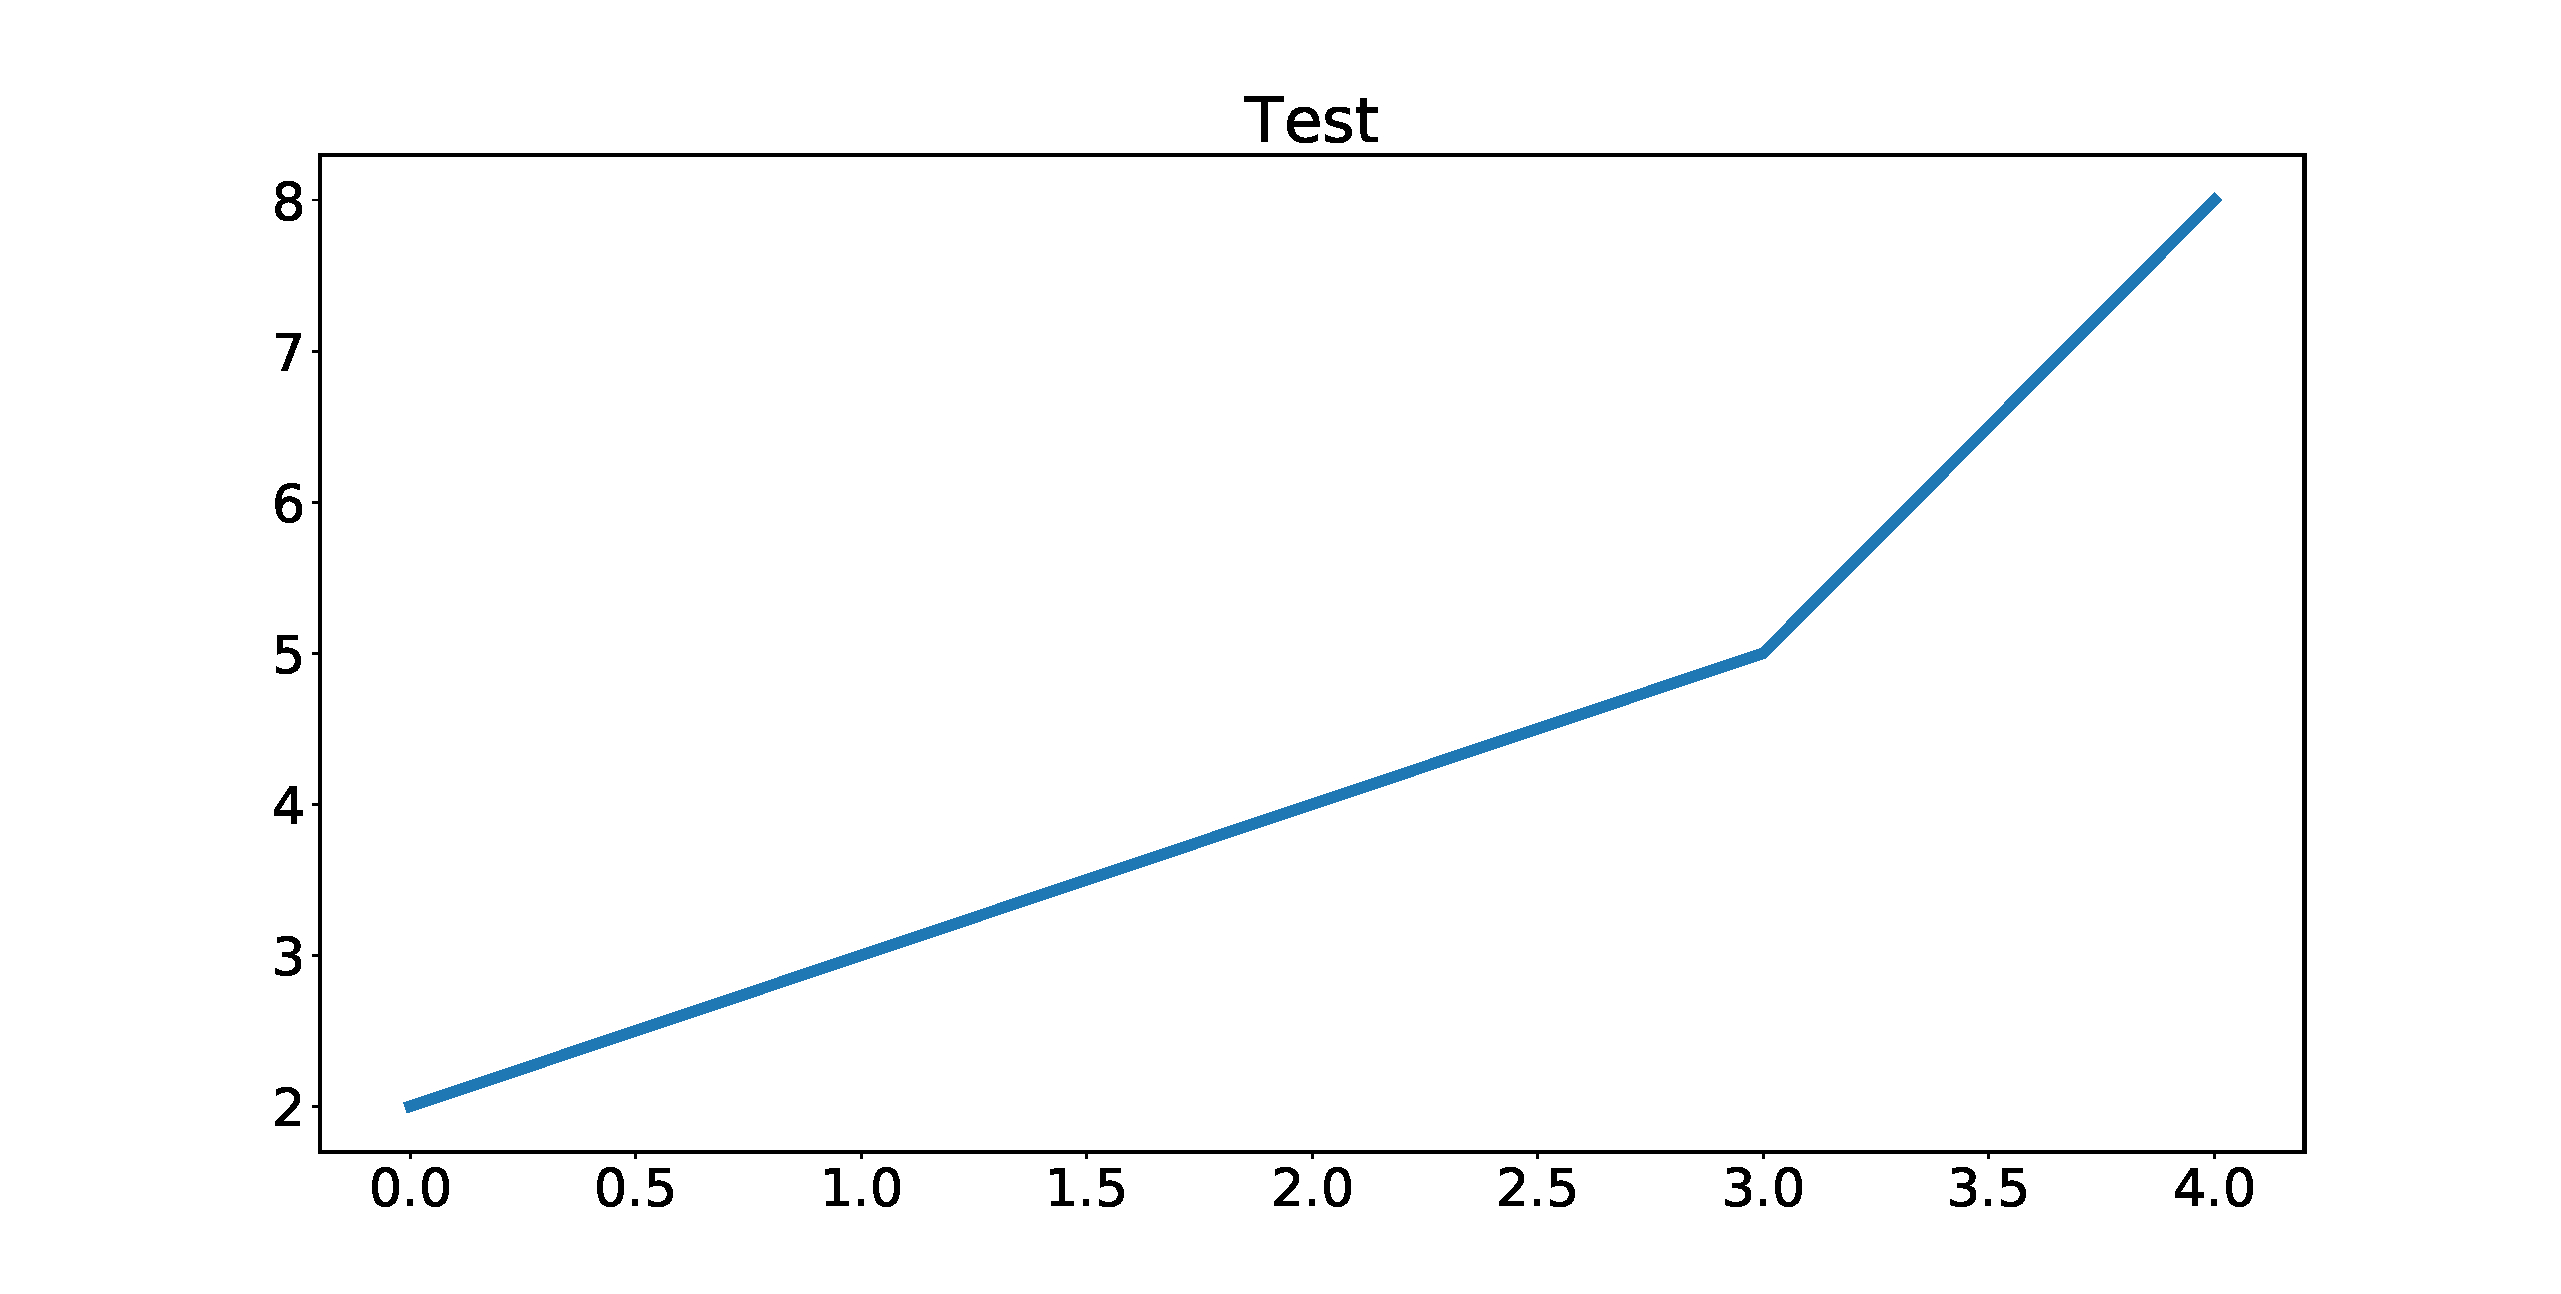
\includegraphics[scale=0.3]{Figure_1.pdf}
\end{figure}

\end{appendices}

\printbibliography

\end{document}
